\documentclass[11pt,a4paper]{scrartcl}
\typearea{12}
\usepackage{graphicx}
\usepackage{pstricks}
\usepackage{listings}
\lstset{language=python}
\pagestyle{headings}
\markright{Computation Neuroscience - Lecture 10}

\usepackage{tikz}
\usepackage{tikzscale}
\usepackage{pgfplots}
\usepackage{color}
\usepackage{pgf}
\usepackage[utf8]{inputenc}
\usetikzlibrary{arrows,automata}
\usetikzlibrary{positioning}


\begin{document}

\subsection*{Features}

Knowing why V1 receptive fields have the particular stucture they do
is likely to tell us something about what it is that the brain does to
information in the sensory pathways. One idea is that it is related to
feature extraction. To motivate this we will consider a ficticious
world of simplified creatures; we are one of these creates and wish to
decide how to react to other creatures we encounter. As in the real
world, when we encounter a creature we need to decide between what are
sometimes called the three Fs: fighting, fleeing and mating. Now
imagine that the creatures all have a three by three pattern on their
stomachs:
\begin{center}
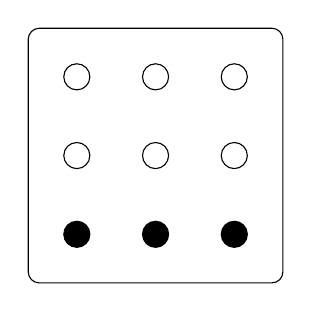
\begin{tikzpicture}
\node[rectangle,rounded corners,draw=black,text width=3cm, text height=3cm](big){};
\node[circle,draw=black, fill=white](a1){};
\node[circle,draw=black, fill=white,right of =a1](b1){};
\node[circle,draw=black, fill=white,left of =a1](c1){};
\node[circle,draw=black, fill=black,below of=a1](a2){};
\node[circle,draw=black, fill=black,right of =a2](b2){};
\node[circle,draw=black, fill=black,left of =a2](c2){};
\node[circle,draw=black, fill=white,above of =a1](a3){};
\node[circle,draw=black, fill=white,right of =a3](b3){};
\node[circle,draw=black, fill=white,left of =a3](c3){};
\end{tikzpicture}
\end{center}
and that creatures to fight have a horizontal strip to the top or the bottom, as above, creatures to flee from, a vertical strip on the left or right, for example
\begin{center}
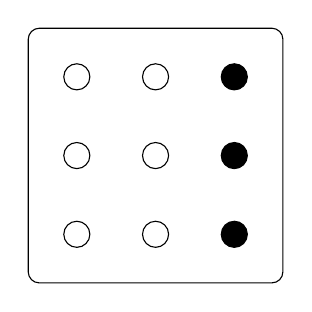
\begin{tikzpicture}
\node[rectangle,rounded corners,draw=black,text width=3cm, text height=3cm](big){};
\node[circle,draw=black, fill=white](a1){};
\node[circle,draw=black, fill=black,right of =a1](b1){};
\node[circle,draw=black, fill=white,left of =a1](c1){};
\node[circle,draw=black, fill=white,below of=a1](a2){};
\node[circle,draw=black, fill=black,right of =a2](b2){};
\node[circle,draw=black, fill=white,left of =a2](c2){};
\node[circle,draw=black, fill=white,above of =a1](a3){};
\node[circle,draw=black, fill=black,right of =a3](b3){};
\node[circle,draw=black, fill=white,left of =a3](c3){};
\end{tikzpicture}
\end{center}
and creatures to mate with, a central line, either horizontal or vertical like:
\begin{center}
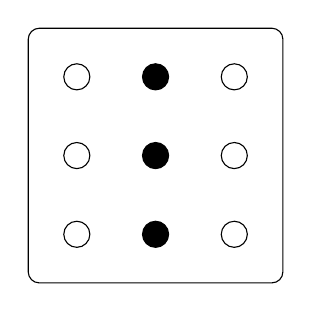
\begin{tikzpicture}
\node[rectangle,rounded corners,draw=black,text width=3cm, text height=3cm](big){};
\node[circle,draw=black, fill=black](a1){};
\node[circle,draw=black, fill=white,right of =a1](b1){};
\node[circle,draw=black, fill=white,left of =a1](c1){};
\node[circle,draw=black, fill=black,below of=a1](a2){};
\node[circle,draw=black, fill=white,right of =a2](b2){};
\node[circle,draw=black, fill=white,left of =a2](c2){};
\node[circle,draw=black, fill=black,above of =a1](a3){};
\node[circle,draw=black, fill=white,right of =a3](b3){};
\node[circle,draw=black, fill=white,left of =a3](c3){};
\end{tikzpicture}
\end{center}

Now, imagine processing this information so as to rapidly decide what
to do, the simplest neural network to process the patterns would look
like
\begin{center}
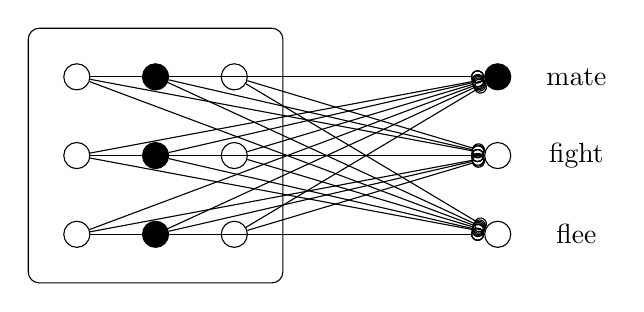
\begin{tikzpicture}
\node[rectangle,rounded corners,draw=black,text width=3cm, text height=3cm](big){};
\node[circle,draw=black, fill=black](a1){};
\node[circle,draw=black, fill=white,right of =a1](b1){};
\node[circle,draw=black, fill=white,left of =a1](c1){};
\node[circle,draw=black, fill=black,below of=a1](a2){};
\node[circle,draw=black, fill=white,right of =a2](b2){};
\node[circle,draw=black, fill=white,left of =a2](c2){};
\node[circle,draw=black, fill=black,above of =a1](a3){};
\node[circle,draw=black, fill=white,right of =a3](b3){};
\node[circle,draw=black, fill=white,left of =a3](c3){};
\node[circle,draw=black,right =3cm of b2](fl){};
\node[circle,draw=black,right =3cm of b1](fi){};
\node[circle,draw=black,right =3cm of b3,fill=black](fu){};
\node[right of=fl](flee){flee};
\node[right of=fi](fight){fight};
\node[right of=fu](mate){mate};
\draw (a1) edge[-o] (fl);
\draw (b1) edge[-o] (fl);
\draw (c1) edge[-o] (fl);
\draw (a2) edge[-o] (fl);
\draw (b2) edge[-o] (fl);
\draw (c2) edge[-o] (fl);
\draw (a3) edge[-o] (fl);
\draw (b3) edge[-o] (fl);
\draw (c3) edge[-o] (fl);
\draw (a1) edge[-o] (fi);
\draw (b1) edge[-o] (fi);
\draw (c1) edge[-o] (fi);
\draw (a2) edge[-o] (fi);
\draw (b2) edge[-o] (fi);
\draw (c2) edge[-o] (fi);
\draw (a3) edge[-o] (fi);
\draw (b3) edge[-o] (fi);
\draw (c3) edge[-o] (fi);
\draw (a1) edge[-o] (fu);
\draw (b1) edge[-o] (fu);
\draw (c1) edge[-o] (fu);
\draw (a2) edge[-o] (fu);
\draw (b2) edge[-o] (fu);
\draw (c2) edge[-o] (fu);
\draw (a3) edge[-o] (fu);
\draw (b3) edge[-o] (fu);
\draw (c3) edge[-o] (fu);
\end{tikzpicture}
\end{center}
Clearly this would be very hard to learn; the connection from, say the
bottom middle node is on in two of the patterns above despite these patterns
corresponding to different types of creature. 

A far better strategy would be to first learn features and then learn
the association between these features and the creature type. Here the features are clearly the horizontal and vertical bars
\begin{center}
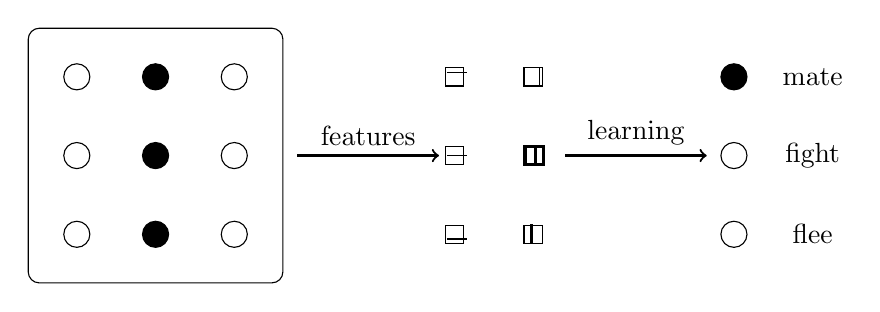
\begin{tikzpicture}
\node[rectangle,rounded corners,draw=black,text width=3cm, text height=3cm](big){};
\node[circle,draw=black, fill=black](a1){};
\node[circle,draw=black, fill=white,right of =a1](b1){};
\node[circle,draw=black, fill=white,left of =a1](c1){};
\node[circle,draw=black, fill=black,below of=a1](a2){};
\node[circle,draw=black, fill=white,right of =a2](b2){};
\node[circle,draw=black, fill=white,left of =a2](c2){};
\node[circle,draw=black, fill=black,above of =a1](a3){};
\node[circle,draw=black, fill=white,right of =a3](b3){};
\node[circle,draw=black, fill=white,left of =a3](c3){};
\node[circle,draw=black,right =6cm of b2](fl){};
\node[circle,draw=black,right =6cm of b1](fi){};
\node[circle,draw=black,right =6cm of b3,fill=black](fu){};
\node[right of=fl](flee){flee};
\node[right of=fi](fight){fight};
\node[right of=fu](mate){mate};
\node[rectangle,draw=black,right=2.5cm of b2](h1){};
\node[rectangle,draw=black,right=2.5cm of b1](h2){};
\node[rectangle,draw=black,right=2.5cm of b3](h3){};
\node[rectangle,draw=black,right=3.5cm of b2](v1){};
\node[rectangle,draw=black,very thick,right=3.5cm of b1](v2){};
\node[rectangle,draw=black,right=3.5cm of b3](v3){};
\draw (3.7,-1.06) -- (3.95,-1.06);
\draw (3.7,1.06) -- (3.95,1.06);
\draw (3.7,0.00) -- (3.95,0.00);
\draw (4.775,-0.875) edge[thick] (4.775,-1.125);
\draw (4.875,0.875) -- (4.875,1.125);
\draw (4.825,-0.125) edge[thick] (4.825,0.125);
\draw (1.8,0) edge[thick,->] node[above]{features} (3.6,0);
\draw (5.2,0) edge[thick,->] node[above]{learning} (7.0,0);
\end{tikzpicture}
\end{center}
In this case the problem has been split in two; first the connections
summarized as \lq{}features\rq{} above are learned from the data,
possibly using the sort of correllation structure learning provided
for by STDP, the interpretation of these feature is then learned, this
is clearly easier, the connections summarized as \lq{}learning\rq{}
have a far simpler task, which is good, since it is crucial to learn
this sort of salient ecological information quickly.


\subsection*{Feature selection}
Here we will consider what properties we would expect features to
have. To do this lets imagine that there are neurons that correspond
to the features and their activity represents the image. Say the
feature neurons each has a receptive field and responds linearly and
for simplicity we will leave out the background firing rate: for the
$s$th feature neuron
\begin{equation}
a_s=\sum_{ij} w^s_{ij}I_{ij}
\end{equation}
and conversely, the output can be represented by
\begin{equation}
I_{ij}=\sum_{s} a^sW^s_{ij}
\end{equation}

The slightly confusing thing here is that we are moving between the linear model and the reconstruction. We do this all the time with vectors:
\begin{equation}
\textbf{v}=v_1\textbf{i}+v_2\textbf{j}+v_3\textbf{k}
\end{equation}
is the reconstruction where the corresponding project, for example
\begin{equation}
v_1-\textbf{v}\cdot\textbf{i}
\end{equation}
is like the linear model. However, the situation in this case is more striaght-forward, because the basis vectors are orthonormal
\begin{equation}
\textbf{i}\cdot\textbf{j}=\textbf{j}\cdot\textbf{k}=\textbf{k}\cdot\textbf{i}=0
\end{equation}
and
\begin{equation}
\textbf{i}\cdot\textbf{i}=\textbf{j}\cdot\textbf{j}=\textbf{k}\cdot\textbf{k}=1
\end{equation}
the same basis vector appears in the reconstruction and the
projection: the coeffient $v_1$ of $\textbf{i}$ in the reconstruction
is the projection of $\textbf{v}$ onto $\textbf{i}$. However, in the
case of vision the basis elements, the $W^s_{ij}$ and $w^s_{ij}$ are
not orthonormal and therefore are not the same, working out the
relationship between involves vectorizing the matrix indices $i$ and
$j$, so we won't go into it here, morally one is the inverse transpose
of the other. In fact, here we will consider an example where the
dimensions are different, where the image patches are $3\times 3$ but
there are only six features, so $s=1\ldots 6$. This means that the
reconstructed image may not be equal the original image and will just
be an approximation to it.

As an example, lets have
\begin{center}
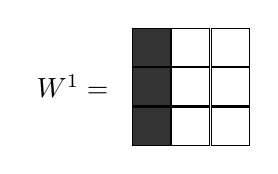
\begin{tikzpicture}
\node at (-1,0.5){$W^1=$};
\node at (0,0)[rectangle,text width=0.25cm,text height=0.25cm,draw=black,fill=black!80,align=center](00){};
\node at (0,0.5)[rectangle,text width=0.25cm,text height=0.25cm,draw=black,fill=black!80,align=center](01){};
\node at (0,1)[rectangle,text width=0.25cm,text height=0.25cm,draw=black,fill=black!80,align=center](02){};
\node at (0.5,0)[rectangle,text width=0.25cm,text height=0.25cm,draw=black,fill=black!0,align=center](10){};
\node at (0.5,0.5)[rectangle,text width=0.25cm,text height=0.25cm,draw=black,fill=black!0,align=center](11){};
\node at (0.5,1)[rectangle,text width=0.25cm,text height=0.25cm,draw=black,fill=black!0,align=center](12){};
\node at (1,0)[rectangle,text width=0.25cm,text height=0.25cm,draw=black,fill=black!0,align=center](20){};
\node at (1,0.5)[rectangle,text width=0.25cm,text height=0.25cm,draw=black,fill=black!0,align=center](21){};
\node at (1,1)[rectangle,text width=0.25cm,text height=0.25cm,draw=black,fill=black!0,align=center](22){};
\end{tikzpicture}
\quad
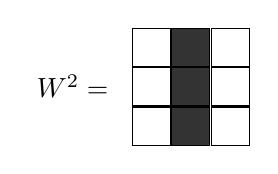
\begin{tikzpicture}
\node at (-1,0.5){$W^2=$};
\node at (0,0)[rectangle,text width=0.25cm,text height=0.25cm,draw=black,fill=black!0,align=center](00){};
\node at (0,0.5)[rectangle,text width=0.25cm,text height=0.25cm,draw=black,fill=black!0,align=center](01){};
\node at (0,1)[rectangle,text width=0.25cm,text height=0.25cm,draw=black,fill=black!0,align=center](02){};
\node at (0.5,0)[rectangle,text width=0.25cm,text height=0.25cm,draw=black,fill=black!80,align=center](10){};
\node at (0.5,0.5)[rectangle,text width=0.25cm,text height=0.25cm,draw=black,fill=black!80,align=center](11){};
\node at (0.5,1)[rectangle,text width=0.25cm,text height=0.25cm,draw=black,fill=black!80,align=center](12){};
\node at (1,0)[rectangle,text width=0.25cm,text height=0.25cm,draw=black,fill=black!0,align=center](20){};
\node at (1,0.5)[rectangle,text width=0.25cm,text height=0.25cm,draw=black,fill=black!0,align=center](21){};
\node at (1,1)[rectangle,text width=0.25cm,text height=0.25cm,draw=black,fill=black!0,align=center](22){};
\end{tikzpicture}
\quad
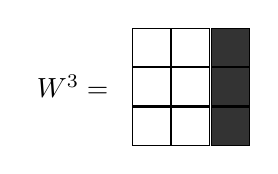
\begin{tikzpicture}
\node at (-1,0.5){$W^3=$};
\node at (0,0)[rectangle,text width=0.25cm,text height=0.25cm,draw=black,fill=black!0,align=center](00){};
\node at (0,0.5)[rectangle,text width=0.25cm,text height=0.25cm,draw=black,fill=black!0,align=center](01){};
\node at (0,1)[rectangle,text width=0.25cm,text height=0.25cm,draw=black,fill=black!0,align=center](02){};
\node at (0.5,0)[rectangle,text width=0.25cm,text height=0.25cm,draw=black,fill=black!0,align=center](10){};
\node at (0.5,0.5)[rectangle,text width=0.25cm,text height=0.25cm,draw=black,fill=black!0,align=center](11){};
\node at (0.5,1)[rectangle,text width=0.25cm,text height=0.25cm,draw=black,fill=black!0,align=center](12){};
\node at (1,0)[rectangle,text width=0.25cm,text height=0.25cm,draw=black,fill=black!80,align=center](20){};
\node at (1,0.5)[rectangle,text width=0.25cm,text height=0.25cm,draw=black,fill=black!80,align=center](21){};
\node at (1,1)[rectangle,text width=0.25cm,text height=0.25cm,draw=black,fill=black!80,align=center](22){};
\end{tikzpicture}
\end{center}
\begin{center}
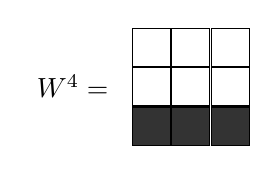
\begin{tikzpicture}
\node at (-1,0.5){$W^4=$};
\node at (0,0)[rectangle,text width=0.25cm,text height=0.25cm,draw=black,fill=black!80,align=center](00){};
\node at (0,0.5)[rectangle,text width=0.25cm,text height=0.25cm,draw=black,fill=black!0,align=center](01){};
\node at (0,1)[rectangle,text width=0.25cm,text height=0.25cm,draw=black,fill=black!0,align=center](02){};
\node at (0.5,0)[rectangle,text width=0.25cm,text height=0.25cm,draw=black,fill=black!80,align=center](10){};
\node at (0.5,0.5)[rectangle,text width=0.25cm,text height=0.25cm,draw=black,fill=black!0,align=center](11){};
\node at (0.5,1)[rectangle,text width=0.25cm,text height=0.25cm,draw=black,fill=black!0,align=center](12){};
\node at (1,0)[rectangle,text width=0.25cm,text height=0.25cm,draw=black,fill=black!80,align=center](20){};
\node at (1,0.5)[rectangle,text width=0.25cm,text height=0.25cm,draw=black,fill=black!0,align=center](21){};
\node at (1,1)[rectangle,text width=0.25cm,text height=0.25cm,draw=black,fill=black!0,align=center](22){};
\end{tikzpicture}
\quad
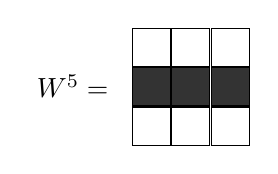
\begin{tikzpicture}
\node at (-1,0.5){$W^5=$};
\node at (0,0)[rectangle,text width=0.25cm,text height=0.25cm,draw=black,fill=black!0,align=center](00){};
\node at (0,0.5)[rectangle,text width=0.25cm,text height=0.25cm,draw=black,fill=black!80,align=center](01){};
\node at (0,1)[rectangle,text width=0.25cm,text height=0.25cm,draw=black,fill=black!0,align=center](02){};
\node at (0.5,0)[rectangle,text width=0.25cm,text height=0.25cm,draw=black,fill=black!0,align=center](10){};
\node at (0.5,0.5)[rectangle,text width=0.25cm,text height=0.25cm,draw=black,fill=black!80,align=center](11){};
\node at (0.5,1)[rectangle,text width=0.25cm,text height=0.25cm,draw=black,fill=black!0,align=center](12){};
\node at (1,0)[rectangle,text width=0.25cm,text height=0.25cm,draw=black,fill=black!0,align=center](20){};
\node at (1,0.5)[rectangle,text width=0.25cm,text height=0.25cm,draw=black,fill=black!80,align=center](21){};
\node at (1,1)[rectangle,text width=0.25cm,text height=0.25cm,draw=black,fill=black!0,align=center](22){};
\end{tikzpicture}
\quad
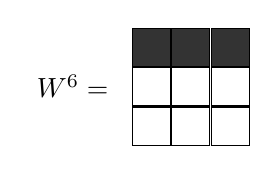
\begin{tikzpicture}
\node at (-1,0.5){$W^6=$};
\node at (0,0)[rectangle,text width=0.25cm,text height=0.25cm,draw=black,fill=black!0,align=center](00){};
\node at (0,0.5)[rectangle,text width=0.25cm,text height=0.25cm,draw=black,fill=black!0,align=center](01){};
\node at (0,1)[rectangle,text width=0.25cm,text height=0.25cm,draw=black,fill=black!80,align=center](02){};
\node at (0.5,0)[rectangle,text width=0.25cm,text height=0.25cm,draw=black,fill=black!0,align=center](10){};
\node at (0.5,0.5)[rectangle,text width=0.25cm,text height=0.25cm,draw=black,fill=black!0,align=center](11){};
\node at (0.5,1)[rectangle,text width=0.25cm,text height=0.25cm,draw=black,fill=black!80,align=center](12){};
\node at (1,0)[rectangle,text width=0.25cm,text height=0.25cm,draw=black,fill=black!0,align=center](20){};
\node at (1,0.5)[rectangle,text width=0.25cm,text height=0.25cm,draw=black,fill=black!0,align=center](21){};
\node at (1,1)[rectangle,text width=0.25cm,text height=0.25cm,draw=black,fill=black!80,align=center](22){};
\end{tikzpicture}
\end{center}
where the almost-black corresponds to one and white to zero, so put another way
\begin{equation}
[W^1_{ij}]=\left(\begin{array}{lll}1&0&0\\1&0&0\\1&0&0\end{array}\right)
\end{equation}
Now consider the example visual input
\begin{center}
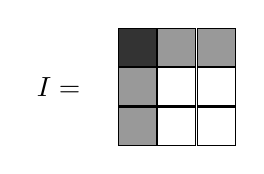
\begin{tikzpicture}
\node at (-1,0.5){$I=$};
\node at (0,0)[rectangle,text width=0.25cm,text height=0.25cm,draw=black,fill=black!40,align=center](00){};
\node at (0,0.5)[rectangle,text width=0.25cm,text height=0.25cm,draw=black,fill=black!40,align=center](01){};
\node at (0,1)[rectangle,text width=0.25cm,text height=0.25cm,draw=black,fill=black!80,align=center](02){};
\node at (0.5,0)[rectangle,text width=0.25cm,text height=0.25cm,draw=black,fill=black!0,align=center](10){};
\node at (0.5,0.5)[rectangle,text width=0.25cm,text height=0.25cm,draw=black,fill=black!0,align=center](11){};
\node at (0.5,1)[rectangle,text width=0.25cm,text height=0.25cm,draw=black,fill=black!40,align=center](12){};
\node at (1,0)[rectangle,text width=0.25cm,text height=0.25cm,draw=black,fill=black!0,align=center](20){};
\node at (1,0.5)[rectangle,text width=0.25cm,text height=0.25cm,draw=black,fill=black!0,align=center](21){};
\node at (1,1)[rectangle,text width=0.25cm,text height=0.25cm,draw=black,fill=black!40,align=center](22){};
\end{tikzpicture}
\end{center}
This would correspond to $a=(0.5,0,0,0,0,0.5)$ or
\begin{center}
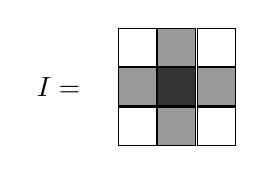
\begin{tikzpicture}
\node at (-1,0.5){$I=$};
\node at (0,0)[rectangle,text width=0.25cm,text height=0.25cm,draw=black,fill=black!0,align=center](00){};
\node at (0,0.5)[rectangle,text width=0.25cm,text height=0.25cm,draw=black,fill=black!40,align=center](01){};
\node at (0,1)[rectangle,text width=0.25cm,text height=0.25cm,draw=black,fill=black!0,align=center](02){};
\node at (0.5,0)[rectangle,text width=0.25cm,text height=0.25cm,draw=black,fill=black!40,align=center](10){};
\node at (0.5,0.5)[rectangle,text width=0.25cm,text height=0.25cm,draw=black,fill=black!80,align=center](11){};
\node at (0.5,1)[rectangle,text width=0.25cm,text height=0.25cm,draw=black,fill=black!40,align=center](12){};
\node at (1,0)[rectangle,text width=0.25cm,text height=0.25cm,draw=black,fill=black!0,align=center](20){};
\node at (1,0.5)[rectangle,text width=0.25cm,text height=0.25cm,draw=black,fill=black!40,align=center](21){};
\node at (1,1)[rectangle,text width=0.25cm,text height=0.25cm,draw=black,fill=black!0,align=center](22){};
\end{tikzpicture}
\end{center}
corresponds to $a=(0,0.5,0,0,0.5,0)$ whereas
\begin{center}
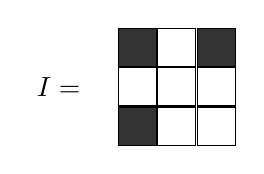
\begin{tikzpicture}
\node at (-1,0.5){$I=$};
\node at (0,0)[rectangle,text width=0.25cm,text height=0.25cm,draw=black,fill=black!80,align=center](00){};
\node at (0,0.5)[rectangle,text width=0.25cm,text height=0.25cm,draw=black,fill=black!0,align=center](01){};
\node at (0,1)[rectangle,text width=0.25cm,text height=0.25cm,draw=black,fill=black!80,align=center](02){};
\node at (0.5,0)[rectangle,text width=0.25cm,text height=0.25cm,draw=black,fill=black!0,align=center](10){};
\node at (0.5,0.5)[rectangle,text width=0.25cm,text height=0.25cm,draw=black,fill=black!0,align=center](11){};
\node at (0.5,1)[rectangle,text width=0.25cm,text height=0.25cm,draw=black,fill=black!0,align=center](12){};
\node at (1,0)[rectangle,text width=0.25cm,text height=0.25cm,draw=black,fill=black!0,align=center](20){};
\node at (1,0.5)[rectangle,text width=0.25cm,text height=0.25cm,draw=black,fill=black!0,align=center](21){};
\node at (1,1)[rectangle,text width=0.25cm,text height=0.25cm,draw=black,fill=black!80,align=center](22){};
\end{tikzpicture}
\end{center}
lies outside the six-dimensional subspace spanned by the features.

The question now is what principle to use to select the features. One
idea, due to \cite{}, is to use sparseness. Going back to the example
with creatures with patterned bellies, looking at flee-from animal,
for example, three dots are black so among neurons that code for
individual dots three would be active, but among neurons coding for
vertical or horizontal lines, only one would be active. 

Of course this is a very artificial made-up example, the it thought
that \lq{}sparseness\rq{} is a good way to define features
\cite{OlshausenField1996a,OlshausenField1997a}. Very roughly, the
fewer neurons needed to reconstruct an image, the more of the image
each neuron is coding for; for this to work without having a vast
number of neurons covering every possible combination of pixels, the
neurons must code for features, piece of image that occur
regularly. The assumption, in short, is that all the images are mostly
made of the same few building blocks.

The idea is as follows, let $I$ be a image and $\tilde{I}$ an approximation to that image formed using features
\begin{equation}
\tilde{I}_{ij}=\sum_{s}a_sW^s_{ij}
\end{equation}
Now $W^s$ could be under-complete, like above, or over-complete, as it
may be in the visual system, or the dimensions could be chosen to match. Either way, even if the basis is not under-complete, $\tilde{I}$ is an approximation because the $a_s$ are not just chosen to give an accurate reconstruction, but to do so in a sparse way; the are chosen to minimize
\begin{equation}
E=\sum_{ij}(I_{ij}-\tilde{I}_{ij})^2+\beta\sum_s f(a_s)
\end{equation}
This has two terms, the first measures the square error between $I$ and $\tilde{I}$, the second is intended as a measure of sparseness, there are different choices possible, one example would be
\begin{equation}
f(x)=\log_2(1+x^2)
\end{equation}
Now, just looking at two dimensions $(1,0)$ gives
\begin{equation}
\sum_sf(a_s)=\log_2{(2)}+\log_2(1)=1
\end{equation}
whereas the less sparse $(1/\sqrt{2},1/\sqrt{2})$, which as a vector
is the same length, gives
\begin{equation}
\sum_sf(a_s)=2\log_2(3/2)=1.17
\end{equation}
which is larger. The $\beta$ here determines the trade-off between
accuracy and sparseness, if $\beta$ is small the square error is more
important, if $\beta$ is big the sparseness is.

The idea now is to take a corpus of image patches and find the best
features, the ones that on average give the lowest values of $E$. The
algorithm proceeds in two stages, for each image patch the $a_s$ are
chosen to minimise $E$ basically by numerically solving the system of differential equations
\begin{equation}
\frac{\partial E}{\partial a_s}=0
\end{equation}
Next, using the results of this calculation for all the images in the
corpus, the features $W^s_{ij}$ are adjusted 
\begin{equation}
W^s_{ij}\rightarrow W^s_{ij}-\eta \frac{\partial \langle E\rangle}{\partial W^s_{ij}}
\end{equation}
where $\eta$ is a learning rate and $\langle E\rangle$ this average
error. This should reduce the average error in the next run through
the corpus. This is repeated until the best features are found. The
details of how $E$ is minimized over possible choices of the $a_s$ and
how to adjust the $W^s_{ij}$ can be found in
\cite{OlshausenField1996a,OlshausenField1997a}. The results are shown
in Fig.~\ref{fig:edges} and, ignoring the complication that these are
not actually the receptive fields, they do clearly resemble the
receptive fields measured from V1.

\begin{figure}
\begin{center}
\includegraphics[width=12cm]{edges.png}
\end{center}
\caption{Sparse filters; the optimal features $W^s_{ij}$ using
  $16\times 16$ image patches cut from a corpus of pictures of the
  American northwest. [From \cite{OlshausenField1996a}].}
\end{figure}

As described, none of this seems very biological, the sparse filters
were discovered using numerical optimization routines. However, there
are biologically plausible implementations using Hebbian learning, see
for example \cite{OReillyMunakata2000a}. There are other approach
which parallel sparseness as a way of distinguishing features, for
example, Infomax, which examines the informativeness of putative features \cite{}.

\begin{thebibliography}{10}
\bibitem{OlshausenField1996a}
Olshausen BA, Field DJ (1996) Emergence of simple-cell receptive field properties by learning a sparse code for natural images. 
\newblock Nature, 381: 607--609.

\bibitem{OlshausenField1997a}
Olshausen BA, Field DJ (1997) Sparse coding with an overcomplete basis set: A strategy employed by V1?. 
\newblock Vision Research 37: 3311--3325.

\bibitem{OReillyMunakata2000a}
O'Reilly RC, Munakata Y (2000) Computational explorations in cognitive neuroscience: Understanding the mind by simulating the brain. 
\newblock MIT Press.

\bibitem{BellSejnowski1995a}
Bell AJ, Sejnowski TJ (1995) An information-maximization approach to blind separation and blind deconvolution. 
\newblock Neural Computation 7: 1129--1159.

\end{thebibliography}

\end{document}

